Et verktøy for å visualisere hvordan gruppens medlemmer står i forhold til hverandre kalles samarbeidsindikatorer. 
Verktøyet er utarbeidet av Are Holden i samarbeid med EiT-staben. 
Dette var et tilbud alle gruppene i landsbyen fikk og testen ble gjennomført av fasilitatorene. 
Undersøkelsen ble gjennomført ved at vi svarte på en rekke spørsmål anonymt, disse svarene ble så grunnlaget for en graf som illustrerer hvordan gruppen ligger an.
Denne grafen belyser områder som gruppen har små, middels eller store utfordringer på. 
For å oppdage eventuell fremgang ble denne testen gjort to ganger iløpet av EiT-kurset. En gang helt i begynnelsen (2. landsbydag) og en gang mot slutten av prosjektet (10. landsbydag). 

\subsection{2. landsbydag}
På grunn av at den første testen ble tatt i en tidlig fase av gruppearbeidet, gir den et godt intrykk av gruppens initielle situasjon. 
På grafen er det to linjer, en heltrukken rød og en en striplet rød. 
Disse linjene markerer grensene på hvor ting blir regnet som store problemer og små problemer. 
\begin{figure}[H]
    \centering
    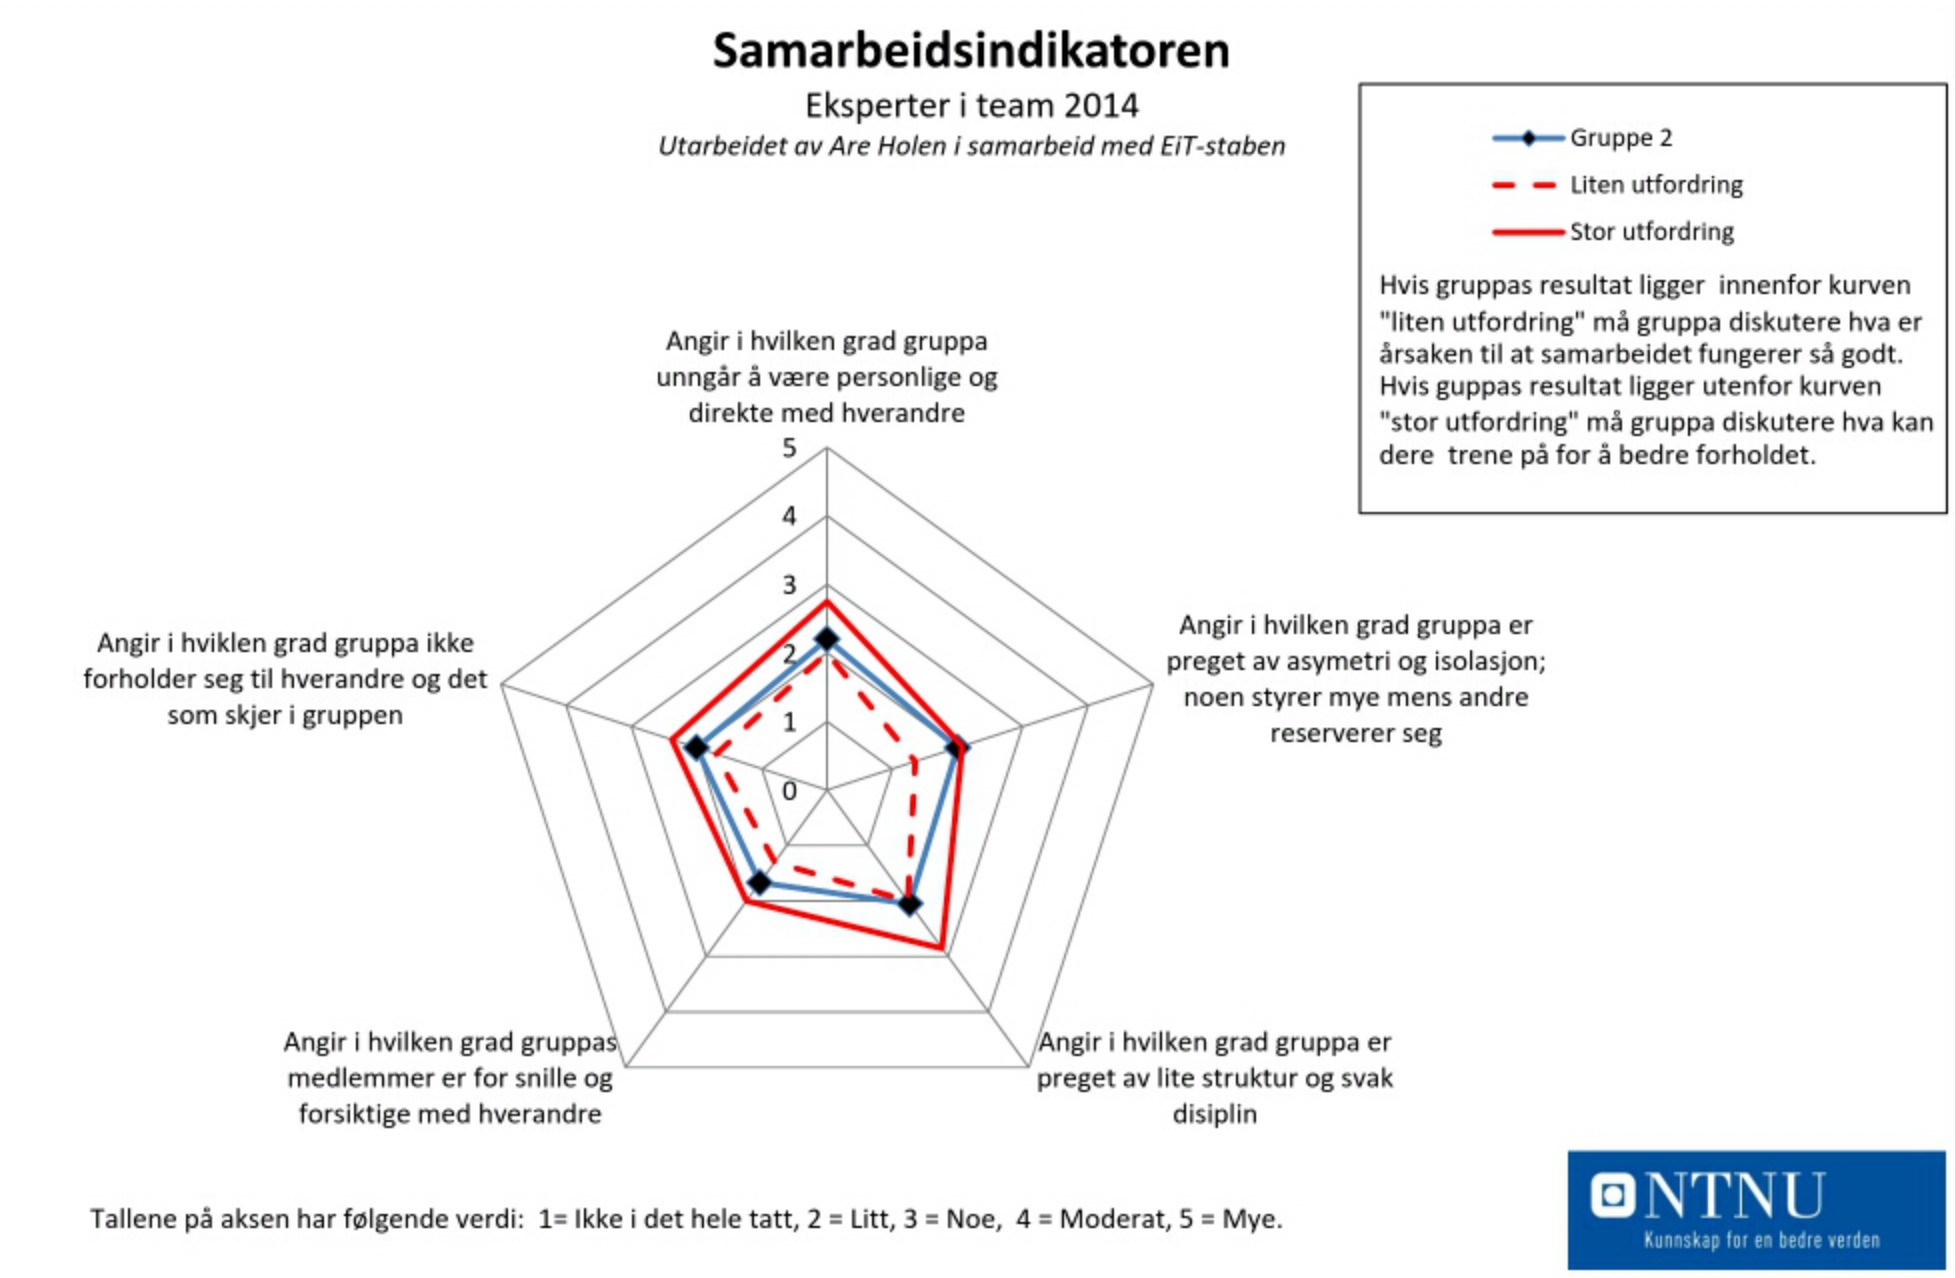
\includegraphics[width=0.7\textwidth]{images/samarbeidsindikator1.jpeg} 
    \caption{Samarbeidsindikatorer 2. landsbydag}
    \label{fig:sam1}
\end{figure}

\noindent \textbf{I hvilken grad gruppen unngår å være personlig:} 2.2.
\newline
\noindent Her hadde vi en moderat utfordring, noe som faller naturlig ettersom vi var en nydannet gruppe.
 At vi selv er bevisste på dette er et godt tegn, noe som gjenspeiler vårt fokus på dette området i videre prosessjobbing.
\vspace{\secspace}

\noindent \textbf{I hvilken grad gruppen er preget av asymetri og isolasjon:} 2.
\newline
\noindent Gruppen hadde de første dagene to medlemmer som var mest dominerende; Odd og Anders.
De tre resterende medlemmene hadde til da tatt en passiv posisjon og var ikke like aktive i felles aktiviterer. 
Under diskusjon av testens resultat, kom vi frem til at dette punktet er noe vi bør jobbe mye med. Vi definerte en aksjon, som var å rullere på å ha lederrollen i gruppa. 
Isolasjon er noe vi følte vi hadde lite av, så det passet dårlig at disse punktene var slått sammen. Vi har hele tiden lagt vekt på at alle i gruppen skal bli hørt, og tas seriøst. 

\vspace{\secspace}

\noindent \textbf{Hvilken grad gruppen er preget av lite struktur:} 1.
\newline
\noindent Som nevnt i punktet over tok noen tak og skapte rammer for arbeidet tidlig i prosessen. Dette gjorde at vi fra begynnelsen jobbet strukturert mot et felles mål. Vi var altså tidlig i prossessen preget av god struktur, og det viste seg i ettertid at grunnarbeidet gjort i den tidlige fasen la grunnlag for en god oppdeling av arbeidet. 
\vspace{\secspace}

\noindent \textbf{Hvilken grad gruppen er for snille med hverandre:} 1.8.
\newline
\noindent Vi kjente hverandre ikke så godt på dette tidspunktet, så dette kan virke naturlig. Vi satte likevel mål om å utvikle en trygghet og respekt for hverandre slik at det blir lettere å være ærlig og konstruktiv.
\vspace{\secspace}

\noindent \textbf{Hvilken grad gruppen ikke forholder seg til hverandre:} 1.
\newline
\noindent Vi hadde fra starten en god tone i gruppa, og ingen meldte seg ut eller ble fryst ut. Indikatoren viser her at dette ikke var et problem i noen særlig grad.

\subsection{10. landsbydag}
\begin{figure}[H]
    \centering
    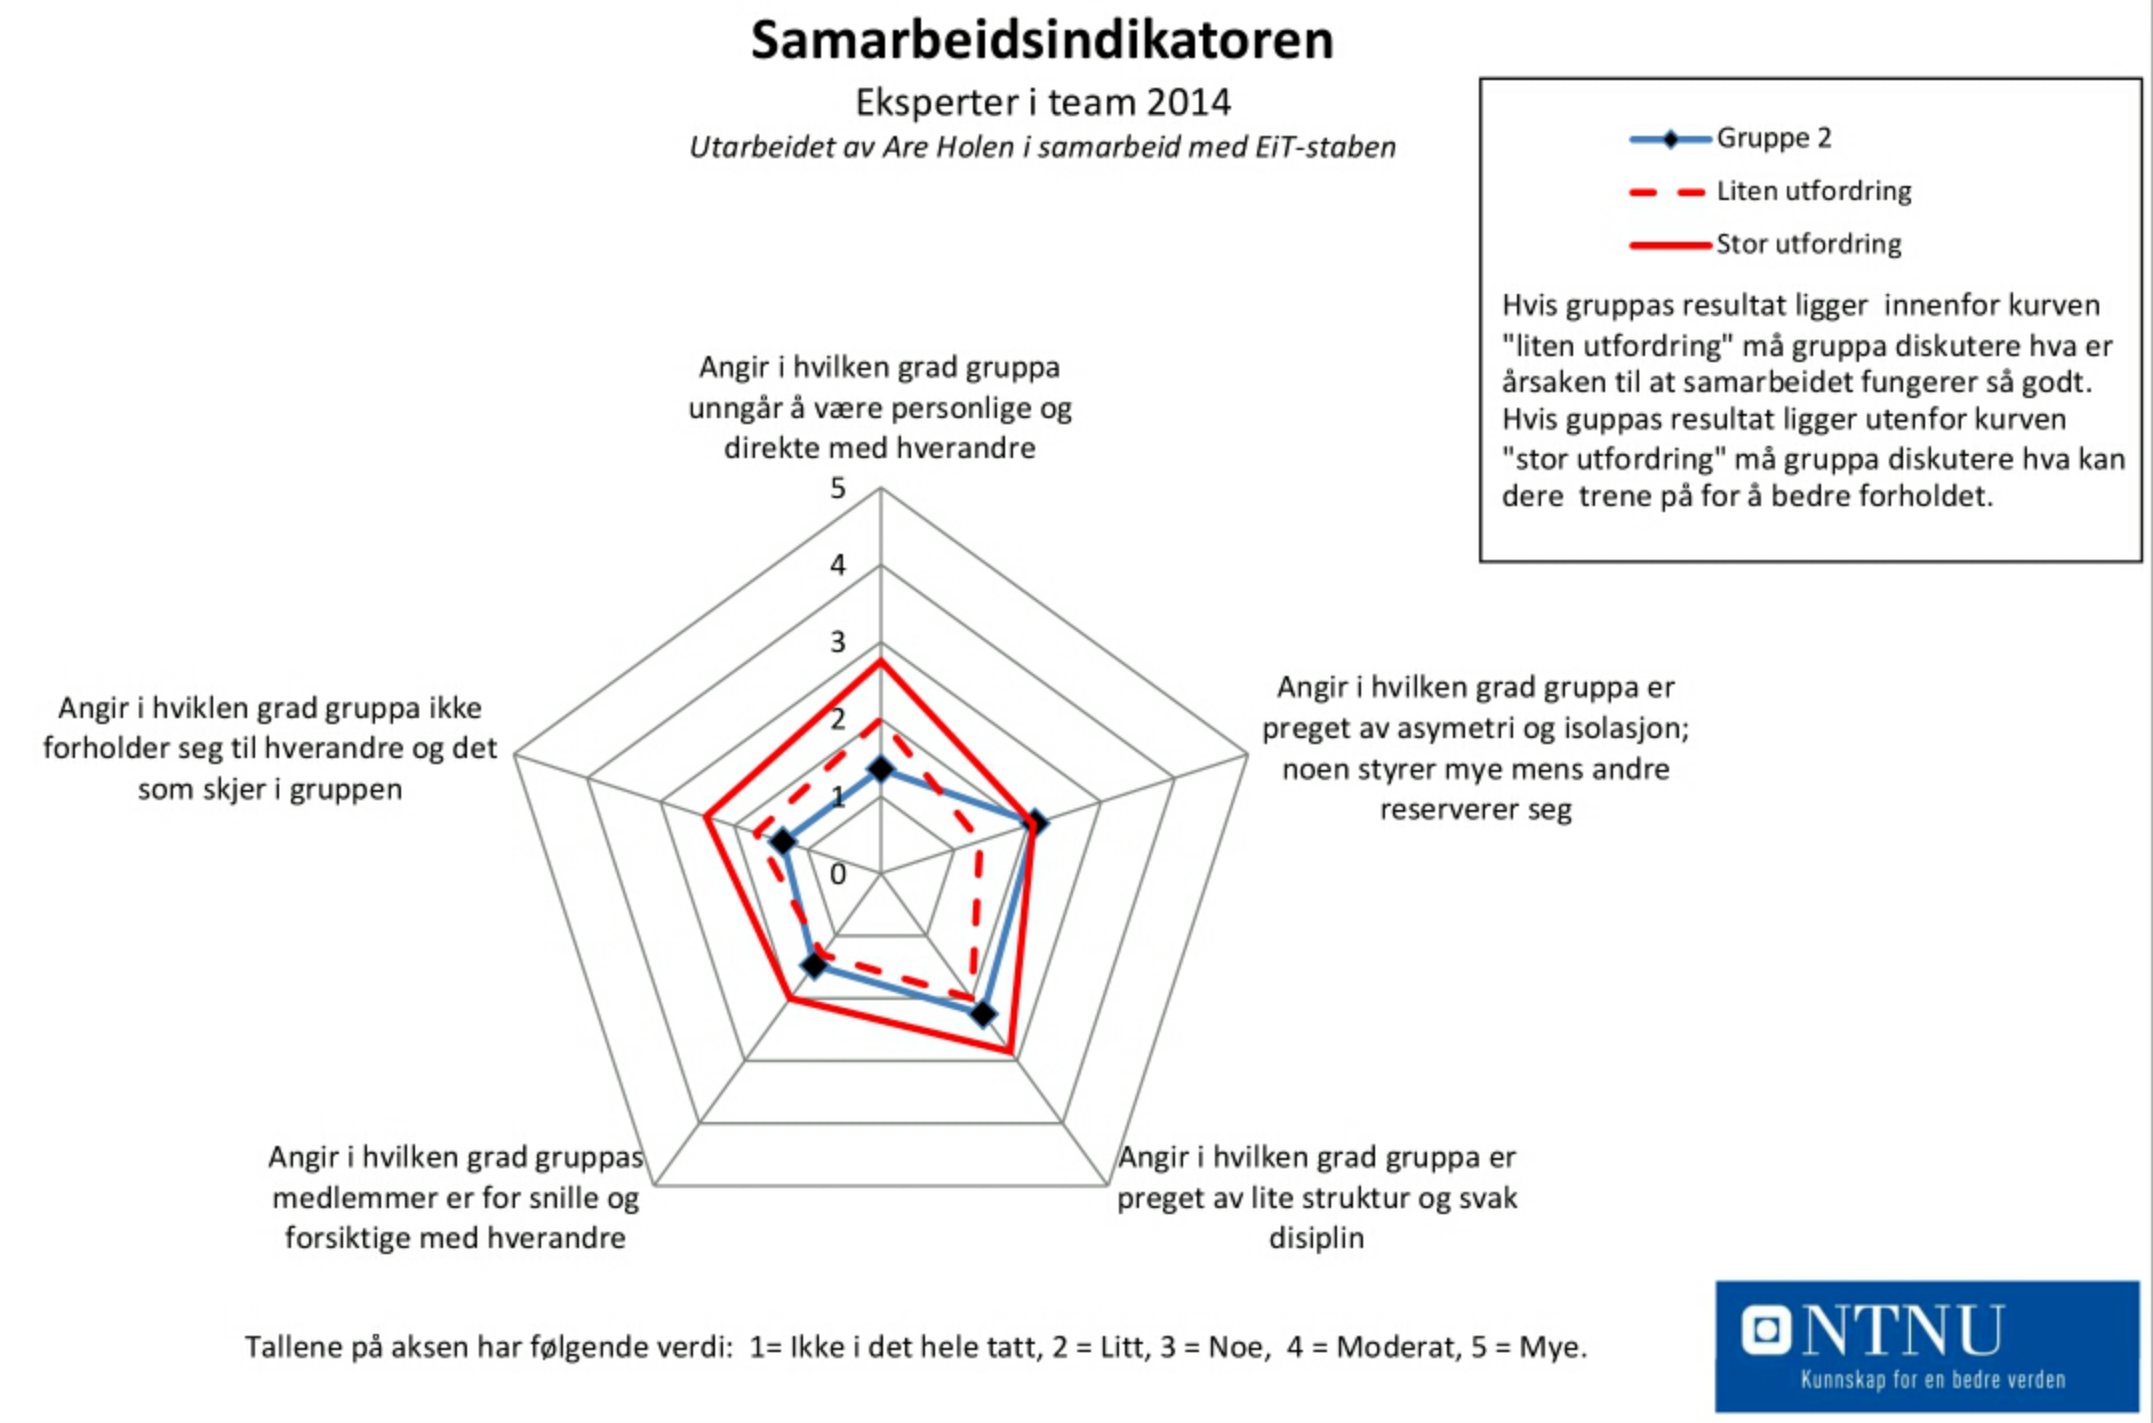
\includegraphics[width=0.7\textwidth]{images/sam2.png} 
    \caption{Samarbeidsindikatorer 10. landsbydag}
    \label{fig:sam2}
\end{figure}

\noindent \textbf{I hvilken grad gruppen unngår å være personlig:} 1.5.
\newline
\noindent Her ser vi en nedgang i forhold til første undersøkelse. Dette gjenspeiler hvordan vi etter hvert har blitt flinkere til å gi ærlige tilbakemeldinger. Hver arbeidsdag har vi brukt 1,5 timer på slutten av dagen til å reflektere over samarbeidet. 
Dette har skapt en arena hvor listen for å ta opp ting er lav, og vi har vært veldig åpne for konstruktiv kritikk.
\vspace{\secspace}

\noindent \textbf{I hvilken grad gruppen er preget av asymetri og isolasjon:} 2.
\newline
\noindent På dette punktet har vi fortsatt en ganske høy verdi. når vi reflekterte over dette resultatet var det ingen som kjente seg igjen i dette. Når det er sagt, så er forsatt aktivitetsnivået i gruppa varierende.
Vi er nå trygge på at de som ønsker å si noe tar ordet, og blir hørt. Hvis man er stille betyr det nå at man er enig, eller ikke har noe spesielt å komme med. I tidligere faser var det kanskje andre grunner til at noen ikke tok ordet. 

\vspace{\secspace}

\noindent \textbf{Hvilken grad gruppen er preget av lite struktur:} 2.2.
\newline
\noindent Vår rullering av lederrollen førte til mange nyttige refleksjoner og erfaringer. 
Samtidig førte det til lite struktur enkelte dager, ettersom graden av lederskap varierte stort fra person til person. For noen var det lett å glemme rollen som leder utover dagen, og falt tilbake i gamle vaner med å trekke seg tilbake. 
Vi opplevde også at gruppen etter hvert begynte å bli litt lei prosjektet, og hadde lettere for å komme med avsporinger.
Prosjektet hadde en god fremgang, og vi så at vi kom til å blir ferdig med det aller meste vi hadde planlagt.
Dette førte til at mye av arbeidslysten minsket.
\vspace{\secspace}

\noindent \textbf{Hvilken grad gruppen er for snille med hverandre:} 1.5.
\newline
\noindent Vi har også her en liten nedgang fra første test. Det at vi ikke enda er fullstendig ærlige og direkte kan forklares av flere ting. 
Rent teknisk har prosjektet vårt gått veldig bra, og kommunikasjonen og samarbeidet har vært godt hele veien. Problemer ved arbeidsmetoder ble jevnlig reflektert over i felleskap, og påfølgende aksjoner ble satt i gang. Vi har altså ikke hatt noen store problemer eller problempersonligheter som har krevd en hardere tone i gruppen. 
\vspace{\secspace}

\noindent \textbf{Hvilken grad gruppen ikke forholder seg til hverandre:} 1.5.
\newline
\noindent Etter hvert som planleggingen var ferdig og den tekniske implementasjonen ble satt i gang, begynte vi å arbeide mer selvstendig. Dette førte til mindre kommunkasjon i en gruppe som helhet, men introduserte heller tettere samarbeid mellom enkelte grupperinger. Vi ser på dette som naturlig i den fasen av arbeidet.
I starten delte vi oss opp på to forskjellige bord for å få plass til alt utstyret vi jobbet med. Etter et par dager hadde vi en grundig diskusjon på om dette var riktig, og kom frem til at vi alle burde sitte rundt samme bord selv om vi jobbet selvstendig, 
Vi reflekterte senere over hvordan dette innvirket på arbeidet vårt. 
Det ble lettere å spørre om små ting man lurte på, vi fikk alle en større innsikt i hva hverandre holdt på med. 
Det var spesielt det at vi ikke satt med ryggen til hverandre, men heller rundt et større bord som var utslagsgivende. 
